\documentclass[../ZF_SWEN1.tex]{subfiles}

\begin{document}

\subsection{Objektorientierung}

\paragraph{Grundidee: } Reale Welt besteht aus Objekten, die untereinander in Beziehungen stehen.

\begin{itemize}
	\item Klasse:
	\begin{itemize}
		\item Daten(Attribute)
		\item Funktionalität(Operationen, Methoden)
	\end{itemize}
	\item Objekte:
	\begin{itemize}
		\item In der Lage Nachrichten (= Methodenaufrufe) zu empfangen
		\item Daten verarbeiten
		\item Nachrichten senden
		\item können einmal erstellt werden
		\item in verschiedene Kontexten wiederverwendet werden
	\end{itemize}
\end{itemize}


\paragraph{Objektorientierte Analyse(OOA): } Objekte-Konzepte-in Domäne zu finden und zu beschreiben. \\
\paragraph{Objektorientierten Design (OOD): } Geeignete Softwareobjekte und ihr Kollaboration zu definieren um Anforderungen zu erfüllen.

\paragraph{Domänenschicht: } Klassen abgeleitet aus dem Domänenmodell (Low-Representational-Gap)


\subsubsection{Use Cases und System-Sequenzdiagramm}
\paragraph{Basis für das Design: }
\begin{enumerate}
	\item Szenarien
	\item Systemoperationen
	\item Domänenmodell
\end{enumerate}

\subparagraph{Was programmiert werden muss: }
\begin{enumerate}
	\item Systemoperationen bzw. deren Antworten
\end{enumerate}


\paragraph{Use-Case-Realisierung: } Wie ein bestimmter Use Case innerhalb Design mit kollaborierenden Objekten realisiert wird.

\paragraph{Systemoperationen: } Jedes Szeanario schrittweise entworfen und implementiert

\paragraph{UML-Diagramme: } Gemeinsame Sprache um Use-Case-Realisierungen zu veranschaulichen und zu diskutieren.


\subsubsection{Klassen entwerfen: }
Zwei arten von Design-Modellen (ergänzen sich und werden parallel erstellt):
\begin{itemize}
	\item Statische Modelle:
	\begin{itemize}
		\item \textcolor {orange}{UML-Klassendiagramm}- Unterstützen Entwurf Paketen, Klassennamen, Atrributen und Methodensignaturen (ohne Methodenkörperd)
	\end{itemize}
	\item Dynamische Modelle:
	\begin{itemize}
		\item \textcolor {orange} {UML-Interaktionsdiagramme} Untersützen Entwurf der Logik, des Verhaltens des Codes und der Methodenkörper.
	\end{itemize}	
\end{itemize}


\subsection{UML-Diagramme für das Design}
\subsubsection{Grundelemente der UML}
\begin{itemize}
	\item Primitiver Datentyp
	\item Literal
	\item Schlüsselwort, Stereotyp
	\item Randbedingung (constraint)
	\item Kommentar
	\item Diagrammrahmen (optional)
\end{itemize}

\begin{figure}[H]
\centering
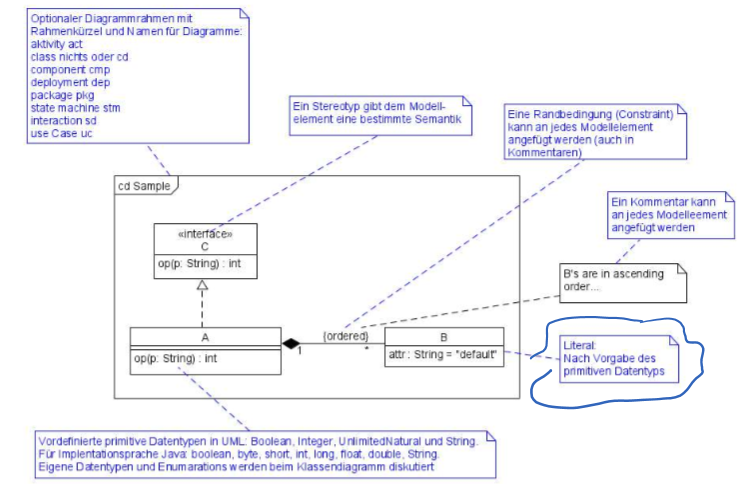
\includegraphics[width=0.3\textwidth]{/Resources/Images/Grundelemente_Klassendiagramm.png}
\caption{\label{fig:Grundelemente_Klassendiagramm}Grundelemente\_Klassendiagramm.}
\end{figure}

\subsubsection{UML-Klassendiagramm}
\begin{itemize}
	\item Statische struktur
	\item Konzeptuell: Problemdomäne (Domänenmodell)
	\item Design: Lösungsdomäne (DCD)
\end{itemize}

\subparagraph{Notationselemente}
\begin{itemize}
	\item Klasse
	\item Attribut
	\item Operation
	\item Sichtbarkeit von Attributen und Operationen
	\item Assoziationsname, Rollen an den Assoziationsenden
	\item Multiplizität (Objekte der betreffenden Klasse)
	\item Navigierbarkeit in Assoziationen
	\item Datentypen und Enumerationen
	\item Generalisierung / Spezialisierung
	\item Abstrakte Klassen
	\item Komposition
	\item Aggregation
	\item Interface
	\item Interface - Realisierung (Menge von öffentlichen Operationen, Merkmalen und Verpflichtungen, die durch eine Klasse, die die Schnittstelle implementiert, zwingend zur Verfügung gestellt werden müssen.
	\item Assoziationsklasse (Da wenn ** Beziehung existiert)
	\item Aktive Klasse (Instanz wird in einem separaten Thread ausgeführt)
\end{itemize}

\subsubsection{UML-Interaktionsdiagramme}

Spezifiziert, auf welche Weise Nachrichten und Daten zwischen Interaktionspartnern ausgetauscht werden. \\

\textcolor {WildStrawberry}{\textbf{2 Arten:}}
\begin{enumerate}
	\item Sequenzdiagramm
	\item Kommunikationsdiagramm
\end{enumerate}

\paragraph{\textcolor {WildStrawberry}{\textbf{Anwendung:}}} Kollaborationen bzw. Informationsaustausch zwischen Objekten zu modellieren.

\begin{itemize}
	\item Wer tauscht mit Wem Information aus?
	\item in welcher Reihenfolge
	\item Zeitlicher Ablauf
	\item Schachtelung und Flussteuerung (Bedingung, Schleifen, Verzweigungen) möglich.
\end{itemize}

\subparagraph{\textcolor {WildStrawberry}{\textbf{Kann in mehreren Perspektiven verwendet werden:}}}
\begin{itemize}
	\item \textcolor {Periwinkle}{Analyse}
	\begin{itemize}
		\item mit SSD Input-/Output-Erignisse (Systemoperationen mit Rückgabeantworten) für ein Szenario eines Use Cases modelliert
	\end{itemize}
	\item \textcolor {Periwinkle}{Design}
	\begin{itemize}
		\item mit SSD Interaktion zwischen Objekten zur Realisierung eines konkreten Use-Case Szenarios zu modellieren
	\end{itemize}
\end{itemize}

\paragraph{Notationselemente:}
\begin{itemize}
	\item Lebenslinie
	\item Aktionssequenz
	\item Synchrone Nachricht
	\item Antwortnachricht
	\item Gefundene, verlorene Nachricht
	\item kombiniertes Fragment
	\item Erzeugnis-, Löschereignis
	\item Selbstaufruf
	\item Interaktionsreferenz
	\item Lebenslinie mit aktiver Klasse
	\item Asynchrone Nachricht
\end{itemize}




	



\subsubsection{UML-Kommunikationsdiagramm}
\paragraph{Beantwortet Frage:}\\
Wer kommuniziert mit werm? Wer arbeitet im System zusammen? Darstellung Informationsaustausch zwischen Kommunikationspartnern. Überblick im Vordergrund.
\paragraph{Notationselemente:}
\begin{itemize}
	\item Lebenslinie (Box)
	\item Synchrone Nachricht (=Aufruf einer Operation)
	\item Antwortnachricht (=Rückgabewert)
	\item Bedingte Nachrichten "[]"
	\item Iteration "*"
	\item Nummerierung der Nachrichten (Festlegung Zeitliche Abfolge)
	\begin{itemize}
		\item Systemoperation (msg1, ohne Nummer)
		\item Nummern gleicher Hierarchie(1,2,3...)
		\item Nummer unterer Hierarchie:
		\begin{itemize}
			\item Werden innerhalb der Operation darüber ausgeführt (verschachtelt)
			\item Operation 1.1:msg3 wird innerhalb von Operation 1:msg2 aufgerufen
		\end{itemize}
	\end{itemize}

\end{itemize}

\subsubsection{UML-Zustandsdiagramm}
\paragraph{Beantwortet zentrale Frage:}\\
Weleche Zustände kann ein Objekt, eine Schnittstelle, ein Use Case, ...bei welchen Ereignissen annehmen?\\
Präzise Abbildung eines Zustandmodells (endlicher Automat):
\begin{itemize}
	\item Zuständen
	\item Ereignissen
	\item Nebenläufigkeiten
	\item Bedingungen
	\item Ein- und Austrittsaktionen
\end{itemize}
\subparagraph{Verwendung:} Modellierung von Echtzeitsystemen, Steuerungen und Protokollen 

\paragraph{Notationselemente:}
\begin{itemize}
	\item Start-, Endzustand
	\item einfacher Zustand
	\item Zusammengesetzter bzw. geschachtelter Zustand
	\item Transition
	\item Orthogonaler Zustand
	\item Parallelisierungsknoten
	\item Synchronisationsknoten
	\item Einstiepunkt
	\item Ausstigespunkt
	\item Unterzustandautomat
	\item Zusammengesetzter Zustand
	\item Flache und tiefe Historie
\end{itemize}


\subsubsection{UML-Aktivitätsdiagramm}
\paragraph{Beantwortet zentrale Frage:}\\
Wie läuft ein bestimmter Prozess oder ein Algortithmus ab?\\
Detaillierte Visualisierung von Abläufen:
\begin{itemize}
	\item Bedingungen
	\item Schleifen
	\item Verweigungen
\end{itemize}

Parallelisierung und Synchronisation von Aktionen möglich.

\paragraph{Notationselemente:}
\begin{itemize}
	\item Aktivität
	\item Aktionsknoten (Aktion)
	\item Objektknoten (Objekt)
	\item Entscheidungs- und Vereinigungsknoten
	\item Initialknoten
	\item Aktivitätsendknoten
	\item Partition / Swimlane
	\item Parallelisierungsknoten
	\item Synchronisationsknoten
	\item SendSignal-Aktion
	\item Ereignis- bzw. Zeitereignisannahmeaktion
	\item CallBehavior-Aktion
\end{itemize}


\subsection{Verantwortlichkeiten und Responsibility-Driven-Design}:
Methode über Entwurf Softwareklassen nachzudenken:
\textcolor {yelloworange} {\textbf{Verantwortlichkeiten, Rollen, Kollaborationsbeziehungen}} = \textbf{RDD / Responsibility Driven Design}\\

Softwareobjekte haben Verantwortlichkeiten und arbeiten mit anderen Objekten zusammen.\\
Verantwortlichkeiten werden durch Attribute und Methoden implementiert.\\
Kann auf jeder Ebene des Designs angwendet werden:
\begin{itemize}
	\item Klasse
	\item Komponente
	\item Schicht
\end{itemize}


\paragraph{2 Ausprägungen von Verantwortlichkeiten:}
\subparagraph{\textcolor {brick}{\textbf{Doing-Verantwortlichkeiten / Algorithmen, Code:}}
\begin{itemize}
	\item Selbst etwas tun
	\item Aktionen anderer Objekte anstossen
	\item Aktivitäten anderer Objekte kontrollieren und steuern
\end{itemize}

\subparagraph{\textcolor {brick}{\textbf{Knowing-Verantwortlichkeit / Daten, Attribute: }}
\begin{itemize}
	\item Private eingekapselte Daten
	\item Dinge kennen, die es ableiten oder berechnen kann
	\item Daten/Objekte zur Verfügung stellen, die aus bekannten Daten/Objekten abgeleitet oder berechnet werden können
\end{itemize}


\subsubsection{GRASP- 9 Patterns}
\begin{enumerate}
	\item \textbf{Information Expert}
	\begin{itemize}
		\item \textcolor {teal} {Derjenige, der was weiss}
	\end{itemize}
	\item \textbf{Creator}
		\begin{itemize}
		\item \textcolor {teal} {Zuständig erstellen Objekte(new())im Framework ABER delegiert als Dependency Injection}
	\end{itemize}
	\item \textbf{Controller /Domain Controller = Service}
	\item \textbf{Low Coupling}
		\begin{itemize}
		\item \textcolor {teal} {Weniger Abhängigkeiten}
	\end{itemize}
	\item \textbf{High Cohesion}
		\begin{itemize}
		\item \textcolor {teal} {Abhängigkeiten zusammentun}
	\end{itemize}
	\item \textbf{Polymorphism}
		\begin{itemize}
		\item \textcolor {teal} {Unterschiedliche Objekte können gleiche Nachricht empfangen und interpretieren}
	\end{itemize}
	\item \textbf{Pure Fabrication}
	\item \textbf{Indirection}
	\item \textbf{Protected Variations}
\end{enumerate}

\subsubsection{Information Expert}

Lösung:\\
Verantwortlichkeit einer Klasse zuweisen, die über die erforderlichen Informationen verfügt, um sie zu erfüllen. Partielle Verantwortlichkeiten sind auch möglich.\\
Alternativen:\\
Low Coupling, High Cohesion (Künstliche Klasse)



\subsubsection{Creator}
Denn Nachteil von new..() = Kopplung\\
Lösung:\\
\textbf {Klasse A} zuständig eine neue Instanz einer \textbf{Klasse B} zu erzeugen, wenn eine oder mehrerere der folgenden Aussagen wahr ist(je mehr desto besser):\\
\begin{itemize}
	\item A eine Aggregation oder ein Kompositum von B
	\item A registriert oder erfasst B-Objekte
	\item A arbeitet eng mit B-Objekten zusammen oder hat enge Kopplung
	\item A verfügt über Initialisierungsdaten für B (A ist Experte bezüglich Erzeugung von B)
\end{itemize}
Wenn mehrere Optionen anwendbar sind, Klasse A vorziehen, die ein Aggregat oder ein Kompositum ist.\\
Alternative:\\
Factory Pattern, Dependency Injection(DI)

\subsubsection{Controller}

Service = 1.Schicht = Domain Controller\\
Welches erste Objekt jenseits der UI-Schicht empfängt und koordiniert(kontrolliert) eine Systemoperation?\\
Lösung:\\
Verantwortlichkeit der Klasse zuweisen, der eine der folgenden Bedingungen erfüllt:\\
\begin{itemize}
	\item Variante 1: Fassaden Controller:
	\begin{itemize}
		\item Repräsentiert "Root-Objekt", System bzw. übergeordnetes System auf dem die Sowftware läuft.
	\end{itemize}
	\item Variante 2: Use Case Controller:
	\begin{itemize}
		\item Pro Use-Case-Szenario eine künstliche Klasse, in der die Systemoperationen abläuft.
	\end{itemize}
\end{itemize}

\textbf{{\large Controller macht selber nur wenig und delegiert fast alles!}}

\begin{figure} [H]
\centering
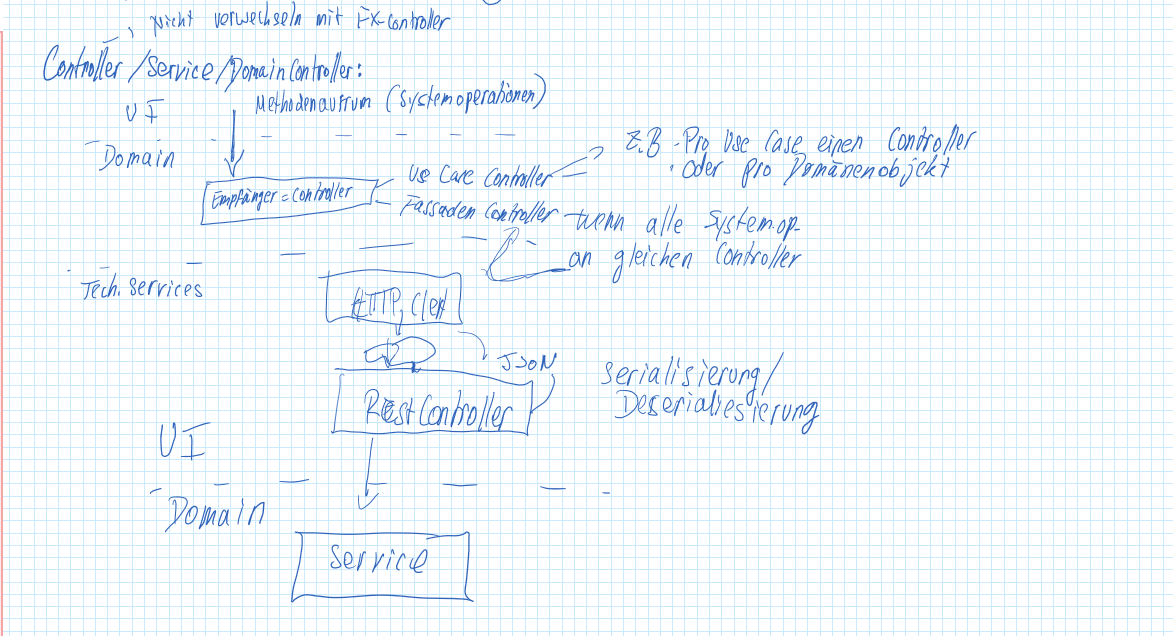
\includegraphics[width=0.3\textwidth]{\Resources\Images\Controller.png}
\caption{\label{fig:Controller}Controller.}

\end{figure}


\subsubsection{Low Coupling}

Ziel: geringe Abhängigkeit (besser für Refactoring)
\begin{itemize}
	\item Kopplung = Mass für die Abhängigkeit von anderen Elementen (Klassen, Subsystem,Systeme)
	\item Hohe Kopplung= Element ist von vielen anderen Elementen abhängig
	\begin{itemize}
		\item Nachteil: Refactoring mühsam, schwieriger zu verstehen, schwieriger wiederzuverwenden
		
	\end{itemize}
	\item Niederige Kopplung = Element ist nur von wenigen anderen Elementen abhängig.
\end{itemize}


Lösung:\\
Verwantwortlichkeiten so zuweisen, dass Kopplung gering bleibt, Delegation Information Expert.

\subsubsection{High Cohesion}

Ziel:\\
Erreichen, dass Objekte fokussiert, verständlich handbar bleiben und nebenbei Low Coupling unterstützen

\begin{itemize}
	\item Kohäsion = Mass für Verwandschaft und Fokussierung eines Elements
	\item Hohe Kohäsion = Element erledigt nur wenige Aufgaben, die eng miteinander verwandt sind
	\item Geringe Kohäsion = Element, das für viele unzusammenhängende Dinge verantwortlich ist
\end{itemize}

Nachteil geringe Kohäsion: Schwierig zu verstehen, schwierig wiederzuverwenden, brüchig und instabil, sind laufend von Änderungen betroffen

Lösung:\\
Verwantwortlichkeiten so zuweisen, dass Kohäsion hoch bleibt.



\subsubsection{Polymorphismus}

Ziel: Typabhängige Alternativen handhaben.
\begin{itemize}
	\item Operation weist viele if-then-else bzw. grosse switch-case Anweisungen auf
	\item Bestimmtes Verhalten (z.B Einsatz eines externen Dienstes konfigurierbar machen.
\end{itemize}

Lösung:\\
Typabhängige Verhalten mit polymorphen Operationen der Klasse zuweisen, dessen Verhalten variiert.
\begin{itemize}
	\item Grundlegende Idee OOP (Generalisierung / Spezialisierung)
	\item Überprüfen dass Beziehung "is a" ist zwischen Superklase und Subklassen
	\item Liskov-Substituions-Prinzip einhalten
\end{itemize}

\subsubsection{Pure Fabrication}
Problem: Wollen nicht gegen High Cohesion und Low Coupling oder andere Ziele verstossen, aber Lösungen nicht passen
\begin{itemize}
	\item Viele Design-Klassen können direkt aus dem Fachbereich (Domänenmodell) abgeleitet werden und erfüllen das Low Representational Gap
	\item viele Situationen wo es Probleme gibt wenn Verantwortlichkeiten der Klasse in der Domänenschicht zugewiesen werden
\end{itemize}

Lösung:\\
\begin{itemize}
	\item Hoch kohäsiven Satz von Verantwortlichkeiten einer künstlichen Hilfsklasse zuweisen
	\item Nur erstellt um höhere Kohäsion, geringe Kopplung oder eine bessere Wiederverwendbarkeit zu realisieren.
\end{itemize}



\subsubsection{Indirection}
Problem: Verantwortlichkeit zuweisen, so dass direkte Kopplung zwischen 2 oder mehrere Objekte vermeidet wird. Objekte Entkoppeln, für geringere Kopplung und Wiederverwendungspotentioal grösser.\\
Ziel: Zwischen Adapter vermittelt\\
Lösung:\\
\begin{itemize}
	\item Verantwortlichkeit einem zwischengeschalteten Objekt zuweisen
	\item Vermittler schafft eine Indirektion zwischen den anderen Komponenten
	\item Alternativen = Protected Variations
	\item GoF Patterns wie Adapter, Bridge, Facade, Observer oder Mediator verwenden dieses Prinzip
	\item viele Indirections sind Pure Fabrications
\end{itemize}

\subsubsection{Protected Variations}

Problem: Objekte, Subsystem und Systeme entwerfen, so dass Veränderungen und Instabilitäten in diesen Elementen keinen Einfluss auf andere Elemente haben.\\
Ziel: Im Vorfeld Erweiterungen vorbereiten für Zukunft.\\

Lösung:\\

Punkte identifizieren, an denen Veränderungen und Instabilitäten zu erwarten sind. Verantwortlichkeiten so zuweisen, dass diese Punkte durch ein stabiles Interface eingekapselt werden.\\
Unterscheidung der Änderungspunkten:
\begin{itemize}
	\item Variationspunkt:
	\begin{itemize}
		\item Veränderung sind sicher(in Anforderung), zwingend PV Konzepte einbauen
		\item Entwicklungspunkt:
		\begin{itemize}
			\item Veränderungen nicht sicher, treffen mit hoher Wahrscheinlichkeit ein, sind nicht in Anforderungen enthalten.
		\end{itemize}
	\end{itemize}
\end{itemize}


Spekulative Anwendungen vermeiden, sonst unnötige Komplexität.











































































\end{document}